\chapter{Life Is Sacred}

This chapter follows the last movement of the Brockwood Park dialogue of 20 May 1976, in which J. Krishnamurti and his interlocutors ask whether the ending of image, thought, time, and sorrow opens onto compassion, silence, and the sacred. There are no validated blackboard equations or diagram frames for this lecture. The mathematical notation below is therefore a disciplined reading aid: it keeps the distinctions in order without pretending that the dialogue was a formal derivation.

\section{The Blank Wall After Discarding Systems}

The lecture begins after a clearing has already taken place. The outsider has listened, has seen through systems, gurus, and prepared meditations, and has understood that the meditator is not separate from meditation. He has been left without future, without past, without image. The result is not triumph. It is a blank wall.

That blank wall is the right starting point. If the old maps of happiness have been put aside, the first question is not whether the argument is elegant. The first question is whether life can be lived from this clearing. Someone asks, in effect, how one is to get out of bed in the morning. The answer is simple only at the practical level: life demands action. We cannot stay in bed because our theories have collapsed.

But action is not yet the whole problem. Much of what we call action is reaction, conformity, or the continuation of the past. The outsider therefore presses the matter further. Has sorrow ended? Is there actual love? Is there compassion, not merely talk about compassion? And, most sharply, has death been understood?

The opening can be recorded as a schematic clearing:
\begin{equation}
\text{systems, gurus, methods, images}
\quad \longrightarrow \quad
\text{discarded}
\quad \longrightarrow \quad
\text{blank wall}.
\end{equation}
This is not a formula for freedom. It is the initial condition of the inquiry. Negation has cleared a space, and now the dialogue asks whether that space is empty mud or an opening into something deeper.

\section{What Dies When the Self Is an Image?}

The first unresolved question is death. The morning dialogue had reached the point where the observer is seen as the observed, and this was spoken of as death. Now the question is tightened: if the self is nothing but an image, what is it that dies?

There is biological death, the ending of the organism. The speakers acknowledge it, but they are not primarily discussing it. They are asking whether the ending of the psychological self-image is death in any deep sense. If the image is fictitious, then the mere ending of the image may seem too trivial. It may be like turning off a television: something stops, but nothing real has died.

The first distinction is therefore:
\begin{equation}
\text{death}_{\mathrm{bio}}
\neq
\text{death}_{\mathrm{psych}}.
\end{equation}
Biological death is the ending of the organism. Psychological death is being investigated as an ending in consciousness: image, thought, memory, psychological time, and the known.

But the dialogue immediately refuses a shallow reduction:
\begin{equation}
\text{death}_{\mathrm{psych}}
\neq
\text{mere ending of image}.
\end{equation}
That inequality is the hinge. The image may end, and that ending may be necessary, but the lecture insists that death must have a much wider significance.

\subsection{Question \& Answer}

\paragraph{Question.}
If the self is an image, and the image ends, what has really died?

\paragraph{Answer.}
At first, only the image has ended. The image has been taken as astonishingly real, so its ending can feel frightening. Yet if it is only an image that ends, the inquiry remains shallow. The dialogue therefore asks for the meaning of death beyond the disappearance of the image.

\paragraph{Working distinction.}
The first three cases can be placed side by side:
\begin{align}
\text{organism ends} &\quad \Rightarrow \quad \text{biological death}, \\
\text{image ends} &\quad \Rightarrow \quad \text{a shallow psychological ending}, \\
\text{known ends} &\quad \Rightarrow \quad \text{the deeper question of death}.
\end{align}
The third line is where the lecture is moving. Death is not yet being defined; it is being opened.

\section{Death as the Ending of the Known}

The next step is to ask what lies behind the image. The dialogue names thought as the maker of images. If the self-image stops but the maker of images continues, then the root has not ended.

The conceptual ladder is:
\begin{equation}
\text{image}
\longrightarrow
\text{image-maker/thought}
\longrightarrow
\text{memory and concepts}
\longrightarrow
\text{psychological time}
\longrightarrow
\text{the known}.
\end{equation}
The arrow means ``the inquiry is led toward,'' not mechanical causation. Krishnamurti is not offering a theory of mind. He is showing why a merely verbal ending is insufficient.

The dialogue then asks why death should matter to the whole of life. The answer is that death, in the psychological sense under examination, means the ending of everything known: the reality built by thought, the concepts, the images, the memories, and the movement of time as the past carrying itself through the present into the future. Clock time remains. Psychological time is the issue.

\begin{align}
\text{clock time} &\neq \text{psychological time}, \\
\text{psychological time} &\sim \text{past meeting the present and carrying on}.
\end{align}
The symbol $\sim$ is deliberate. We are not defining time in general. We are marking the use of the term inside this dialogue.

\begin{proposition}
In this lecture, death becomes significant only when it is not restricted to biological ending or image-ending, but is understood as the ending of the psychological known.
\end{proposition}

\begin{proof}
The dialogue first distinguishes biological death from the death under discussion. It then tests the ending of image and rejects it as too shallow. It next identifies thought as the image-maker, and includes memory, concept, and psychological time in the field that must end. Therefore the significant sense of death is not the mere disappearance of an image, but the ending of accumulated psychological continuity.
\end{proof}

The distinction can be kept compactly in a pocket-safe table:
\begin{table}
\centering
\begin{tabular}{p{0.30\linewidth}p{0.60\linewidth}}
\hline
\textbf{Term} & \textbf{Use in the dialogue} \\
\hline
Biological death & The organism ends through age, disease, accident, or natural limit. \\
Death of image & The self-image ends; this is necessary but called shallow if taken alone. \\
Ending of thought & The image-maker is seen; still not the whole depth of death. \\
Ending of time & Psychological continuity stops: past no longer projects itself as future. \\
Ending of sorrow & Not merely the end of personal self-pity, but the ending of deeper sorrow in insight. \\
The sacred & Not made by thought, not an image, not an object for examination. \\
\hline
\end{tabular}
\caption{Transcript-backed distinctions. The table is a reading aid, not a system imposed on the dialogue.}
\end{table}

\section{The Stream of Image-Making}

At this point the inquiry changes scale. If the organism dies while image-making remains, does that image-making simply vanish with one brain? The dialogue suggests not. My image and your image may have different frills and colors, but essentially they belong to the same stream. The image is not fundamentally private.

This is an important transition. The problem is no longer only ``my'' self-image. There is a constant flow of image-making. It manifests through people. It is not described as merely one person's possession.

\begin{figure}
\centering
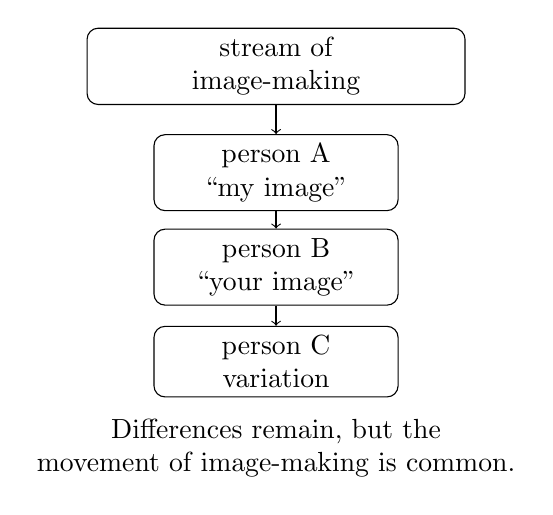
\begin{tikzpicture}[x=1cm,y=1cm]
\node[draw, rounded corners, align=center, minimum width=4.8cm, minimum height=0.85cm] (stream) at (0,0) {stream of\\ image-making};
\node[draw, rounded corners, align=center, minimum width=3.1cm, minimum height=0.75cm] (p1) at (0,-1.35) {person A\\ ``my image''};
\node[draw, rounded corners, align=center, minimum width=3.1cm, minimum height=0.75cm] (p2) at (0,-2.55) {person B\\ ``your image''};
\node[draw, rounded corners, align=center, minimum width=3.1cm, minimum height=0.75cm] (p3) at (0,-3.75) {person C\\ variation};
\draw[->] (stream) -- (p1);
\draw[->] (p1) -- (p2);
\draw[->] (p2) -- (p3);
\node[align=center] at (0,-4.85) {Differences remain, but the\\ movement of image-making is common.};
\end{tikzpicture}
\caption{A narrow schematic reconstruction from the dialogue's river language: image-making is treated as a common stream manifesting through persons.}
\end{figure}

The payoff is that death cannot be understood if we remain confined to the private image. If the individual image is a small manifestation of a larger movement, then the ending of one image is still not the whole of death. The inquiry must move into the stream itself.

\section{Universal Sorrow Beneath the Surface}

The stream metaphor now deepens. Image-making is described as surface movement, like waves on a river. Beneath it is sorrow. This sorrow is not merely pain, not merely loss, not merely the grief of losing a parent or child, and not merely self-pity. It is said to be deeper than thought and ordinary feeling.

The distinction is:
\begin{equation}
\text{sorrow}_{\mathrm{thought}}
\neq
\text{universal sorrow}.
\end{equation}
Thought-made sorrow includes self-pity and the personal drama of the image. Universal sorrow is the deeper sorrow of mankind: ignorance, destruction, repeated wars, poverty, and the long continuity of human beings mistreating one another.

The dialogue asks whether the stream of sorrow is different from the stream of image-making. The answer is subtle. It is not a second stream. It is the same stream at a deeper level. Image-making is the surface wave; sorrow is the depth out of which the surface disturbance comes.

\begin{figure}
\centering
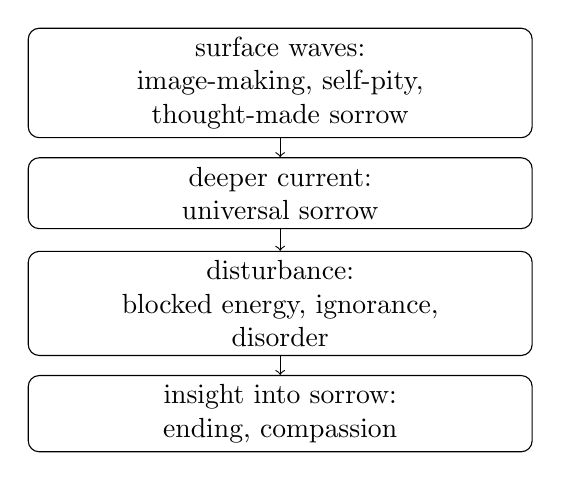
\begin{tikzpicture}[x=1cm,y=1cm]
\node[draw, rounded corners, align=center, minimum width=6.4cm, minimum height=0.75cm] (waves) at (0,1.4) {surface waves:\\ image-making, self-pity,\\ thought-made sorrow};
\node[draw, rounded corners, align=center, minimum width=6.4cm, minimum height=0.75cm] (stream) at (0,0) {deeper current:\\ universal sorrow};
\node[draw, rounded corners, align=center, minimum width=6.4cm, minimum height=0.75cm] (disturb) at (0,-1.4) {disturbance:\\ blocked energy, ignorance,\\ disorder};
\node[draw, rounded corners, align=center, minimum width=6.4cm, minimum height=0.75cm] (insight) at (0,-2.8) {insight into sorrow:\\ ending, compassion};
\draw[->] (waves) -- (stream);
\draw[->] (stream) -- (disturb);
\draw[->] (disturb) -- (insight);
\end{tikzpicture}
\caption{A pocket-size schematic of the stream metaphor. It is not a physical model; it records the dialogue's order of distinctions.}
\end{figure}

\subsection{Question \& Answer}

\paragraph{Question.}
Is universal sorrow a different stream from image-making?

\paragraph{Answer.}
No. The dialogue treats it as part of the same stream, but much deeper. Image-making is surface wave activity. The sorrow of mankind is the deeper current. Disturbances in that depth show themselves at the surface as image, self-pity, fear, anxiety, and confusion.

\paragraph{Worked example.}
Let
\begin{align}
W &= \text{surface waves: image-making and self-pity}, \\
D &= \text{deeper current: universal sorrow}.
\end{align}
A shallow account studies only $W$. The dialogue insists that the serious inquiry must not stop there:
\begin{equation}
W \subset \text{movement of the stream},
\qquad
D \subset \text{movement of the stream},
\qquad
D \text{ is deeper than } W.
\end{equation}
The notation is only a reading aid. Its purpose is to keep universal sorrow from being flattened into private unhappiness.

There is another puzzle. If universal sorrow ends, why does it still exist in mankind? The dialogue resolves this as a problem of language. In insight, sorrow ends for the one who sees; as a wider human fact, sorrow still goes on. Thus:
\begin{equation}
\text{insight into universal sorrow}
\longrightarrow
\text{sorrow ends in that seeing},
\end{equation}
while the disorder of mankind is not thereby magically erased as an external fact.

\section{Compassion and the Corrected Sequence}

The lecture now asks what compassion is. The word is linked with love, but it is handled with great care. Compassion is not pity. It is not sentimental sorrow for another person. It is not the result of passing personally through every horror of mankind.

The tempting formula is:
\begin{equation}
\text{sorrow} \longrightarrow \text{compassion}.
\end{equation}
The dialogue corrects that formula. It would imply that one must go through sorrow first, as though suffering were a method. That implication is rejected. The more precise form is:
\begin{equation}
\text{ending of deeper sorrow}
\longrightarrow
\text{compassion}
\longrightarrow
\text{energy}.
\end{equation}
Even here the arrow must be read cautiously. It does not prescribe a technique. It records the way the discussion clarifies the relation.

\subsection{Question \& Answer}

\paragraph{Question.}
Must one first suffer in order to have compassion?

\paragraph{Answer.}
No. The lecture rejects that sequence. One need not pass through all the horrors of mankind as a personal curriculum. A mind caught in thought-made sorrow, self-pity, and image cannot have compassion. When the deeper sorrow ends, there is compassion.

\paragraph{Careful formulation.}
The phrase ``compassion is born of sorrow'' is safe only if we hear it as:
\begin{equation}
\text{when deeper sorrow ends, compassion is}.
\end{equation}
It is not:
\begin{equation}
\text{personal suffering first, compassion later}.
\end{equation}

The dialogue then uses the image of energy caught in whirlpools, or a vast reservoir of sorrow moving in disorder. This should not be over-modeled. It means that deep sorrow is not a calm object inspected from outside. It is a disorder in the movement of life, perpetuating ignorance. If it were not for that disorder, perhaps mankind's natural capacity to learn would resolve its problems.

\section{Silence, Emptiness, Energy, and the Sacred}

The lecture now returns to death, but death has widened. It is not only the ending of the organism, nor only the ending of image, nor only the ending of the superficial content of consciousness. The speakers ask whether there is something beyond death. The word ``eternal'' is approached and then held back; the more careful phrase is ``beyond time.''

The distinction is:
\begin{equation}
\text{movement in time}
\neq
\text{movement beyond time}.
\end{equation}
Movement in time belongs to duration, transition, and continuity. The other movement is described as constant renewal, freshness, and flowering without becoming old. It is not stored as memory and then altered and called new.

To penetrate into this, the mind must be completely silent. But silence is not produced by control. It is not wished for, premeditated, predetermined, or brought about through will. Otherwise the mind would merely project something into the unknown.

The sequence is:
\begin{equation}
\text{absolute silence}
\longrightarrow
\text{nothing}
\longrightarrow
\text{emptiness}
\longrightarrow
\text{tremendous energy}.
\end{equation}
Then comes an important correction. One speaker asks whether this is the source of compassion. The answer does not settle for the language of source. The stronger statement is:
\begin{equation}
\text{energy} = \text{compassion}.
\end{equation}
This is not physics. Energy here is not measurable energy. It names the living intensity present when the mind is empty of projection, control, image, and psychological time.

From compassion the dialogue asks whether there is something beyond. The answer is the sacred. But the sacred is approached negatively. Everything thought has created is not sacred. An image of worship, whether made by the hand or by the mind, remains an image. Thought is fragmented, limited, finite, and memory-bound; therefore what thought creates cannot be the sacred.

\begin{align}
\text{thought-created sacred} &= \varnothing, \\
\text{sacred} &\notin \text{products of thought}.
\end{align}
The first line is not literal set theory. It is a warning: do not mistake thought's object for the sacred.

The dialogue then asks about relationship. Reality, in the restricted sense of what thought has made, has no relation to the sacred. Relationship comes, if at all, through insight, intelligence, and compassion. Intelligence here is not cleverness. It is insight that is not yours or mine.

\begin{equation}
\text{insight}
\longrightarrow
\text{intelligence}
\longrightarrow
\text{compassion}
\longrightarrow
\text{sacred}.
\end{equation}
The last arrow is delicate. The sacred is not an object reached by a procedure. Krishnamurti says that a living thing cannot be examined as a dead thing. The arrow is therefore a reading aid, not a method.

\section{The Question of Sharing}

The close of the lecture is not a decorative ending. It tests the whole inquiry. What has the viewer actually received? Has the bowl been filled with the sacred, or has the viewer been left with ashes? Has the dialogue shared the perfume of the thing, or only words about it?

The final identification is stark:
\begin{equation}
\text{life} = \text{sacred}.
\end{equation}
This, too, is not offered as a theory. The dialogue immediately warns that accepting it as a theory is no better than accepting any other theory. If life is sacred, then life must not be misused or wasted. Each life is part of the whole.

\subsection{Question \& Answer}

\paragraph{Question.}
Has the dialogue shared the sacred, or only talked about it?

\paragraph{Answer.}
That is the burning question at the end. If the dialogue is only clever argument, nothing essential has been shared. But if the dialogue itself has been meditation, then sharing is no longer one person handing something to another. The final movement points beyond speaker, viewer, and possession: there is only that.

\paragraph{Final reading.}
Meditation is not treated here as a technique added to life. It is the quality of seeing the truth or falseness of each statement as it appears. In that sense the dialogue itself has been the meditation, and its closing claim is not that we have acquired an idea about the sacred, but that the division between observer, viewer, and thing seen has lost its authority.

\section{Summary}

The lecture moves by refusing premature closure. The ending of systems leaves a blank wall. The ending of image is not yet death. The ending of thought is still not deep enough. The stream of image-making leads into the deeper current of sorrow. The ending of deeper sorrow is compassion, and compassion is energy.

Silence, not produced by will, opens into nothing, emptiness, and tremendous energy. The sacred is not made by thought, not captured by an image, and not examined as an object. The dialogue ends by asking whether all this has been shared as living meditation or merely discussed. Its final claim is not a consoling idea about happiness. It is the severe identification that life is sacred, and that to treat this as a theory is already to miss it.